\documentclass{book}
\usepackage{import}
\import{/home/vatican/livreto-liturgico/Sancte-Ioseph/modules/}{def-packages}
\import{/home/vatican/livreto-liturgico/Sancte-Ioseph/modules/}{def-macros}
\import{/home/vatican/livreto-liturgico/Sancte-Ioseph/modules/}{def-pages}
\geometry{a5paper,hdivide={1cm,*,1cm},vdivide={1cm,*,1cm}}
\begin{document}
\begin{center}
    \LARGE Arquidiocese de Olinda e Recife
    \vspace{.2cm} \\
    \Large Paróquia São José
    \vspace{2cm} \\
    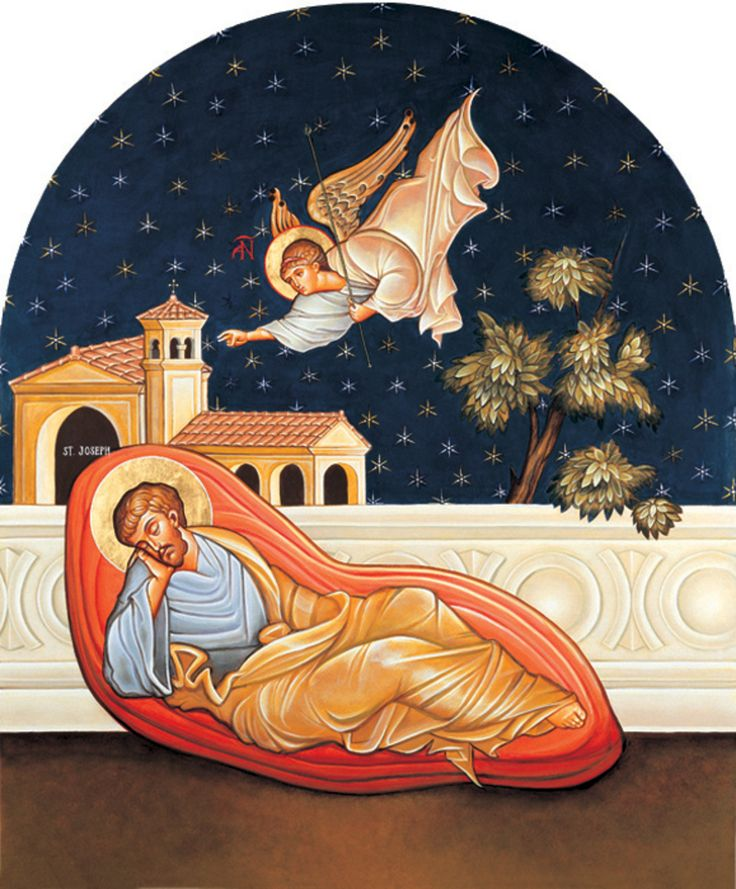
\includegraphics[scale=0.4]{/home/vatican/livreto-liturgico/Sancte-Ioseph/src/joseph.jpeg}
    \vspace{\fill}\\
    \Large Olinda, 18 de Março de 2024
\end{center}
\newpage
\begin{center}
    \LARGE Arquidiocese de Olinda e Recife
    \vspace{.2cm} \\
    \Large Paróquia São José
    \vspace{5cm} \\
    \textcolor{VioletRed2}{\huge Solenidade de São José \\ Esposo da Bem-Aventurada Virgem Maria}
    \vspace{5cm} \\
    \Large Santa Missa Presidida pelo Ex.mo Rev.mo
    \vspace{.2cm} \\
    \textcolor{VioletRed2}{\huge Dom Paulo Jackson}
    \vspace{.2cm} \\
    \Large Arcebispo de Olinda e Recife
    \vspace{.5cm} \\
    \Large Posse do pároco Rev.mo Pe. Charles Araújo
    \vspace{.2cm}
    \vspace{\fill}\\
    \Large Olinda, 18 de Março de 2024
\end{center}

\newpage
\begin{center}
    \textbf{Ritos Iniciais}
\end{center}
\begin{flushleft}
    \textcolor{VioletRed2}{Canto de Entrada}
    \vspace{.2cm} \\
    \textbf{Ergamos os louvores ao justo, a São José, que do alto entre esplendores dirige a nossa fé. Que a ele na fulgência da celestial mansão se eleve toda a ardência de nossa devoção.}
    \vspace{.2cm} \\
    1. Vós sois o casto esposo glorioso de Maria. Vós sois o sol formoso que as almas alumia. \\
    2. Vós sois nossa riqueza, sois da paciência o exemplo. Vós sois a fortaleza, sois da justiça o exemplo. \\
    3. Guardião da virgindade, a fraude tornais vã. Família e sociedade guiais na fé cristã. \\
    4. Sublime, nos altares o vosso amor viceja. De males e pesares, livrando a santa igreja.
    \vspace{.2cm} \\
    \textcolor{VioletRed2}{Saudação}
    \vspace{.2cm}\\
    Em nome do Pai e do Filho e do Espírito Santo. \\
    {\color{VioletRed2} \Rbar.} Amém. \\
    A paz esteja convosco. \\
    {\color{VioletRed2} \Rbar.} Bendito seja Deus \\
    que nos reuniu no amor de Cristo.
    \vspace{.2cm} \\
    \textcolor{VioletRed2}{Leitura do Decreto de Nomeação do Novo Pároco}
    \vspace{.2cm} \\
    \textcolor{VioletRed2}{Ato Penitencial}
    \vspace{.2cm} \\
    Em Jesus Cristo, o Justo, \\
    que intercede por nós e nos reconcilia com o Pai, \\
    abramos o nosso espírito ao arrependimento \\
    para sermos dignos de nos aproximar da mesa do Senhor.
    \vspace{.2cm} \\
    1. Senhor, que na cruz perdoastes o ladrão arrependido, \\
    tende piedade de nós.
    \vspace{.2cm} \\
    \textbf{Kyrie, Kyrie, Kyrie eleison.}
    \vspace{.2cm} \\
    2. Cristo, que nos mandastes perdoar-nos mutuamente antes de nos aproximar do vosso altar, \\
    tende piedade de nós.
    \vspace{.2cm} \\
    \textbf{Christe, Christe, Christe eleison.}
    \vspace{.2cm} \\
    3. Senhor, que confiastes à vossa Igreja o ministério da reconciliação, \\
    tende piedade de nós.
    \vspace{.2cm} \\
    \textbf{Kyrie, Kyrie, Kyrie eleison.}
    \vspace{.2cm} \\
    Deus todo-poderoso tenha compaixão de nós, \\
    perdoe os nossos pecados \\
    e nos conduz à vida eterna. \\
    {\color{VioletRed2} \Rbar.} Amém.
    \vspace{.2cm} \\
    \textcolor{VioletRed2}{Glória}
    \vspace{.2cm} \\
    \textbf{Gloria, Gloria in excelsis Deo. (bis)}
    \vspace{.2cm} \\
    E paz na terra aos homens por Ele amados. \\
    Senhor Deus, rei dos céus, Deus Pai todo poderoso: \\
    Nós vos louvamos, nós vos bendizemos, \\
    nós vos adoramos, nós vos glorificamos, \\
    nós vos damos graças por vossa imensa gloria.
    \vspace{.2cm} \\
    Senhor Jesus Cristo, Filho Unigênito, \\
    Senhor Deus, Cordeiro de Deus, Filho de Deus Pai: \\
    Vós que tirais o pecado do mundo, tende piedade \\
    de nós. Vós que tirais o pecado do mundo, acolhei \\
    a nossa súplica. Vós que estais à direita do Pai, \\
    tende piedade de nós.
    \vspace{.2cm} \\
    Só vós sois o Santo, só vós o Senhor, só vós o \\
    altíssimo, Jesus Cristo, com o Espírito Santo na \\
    gloria de Deus Pai. Amém.
    \vspace{.2cm} \\
    \textcolor{VioletRed2}{Coleta}
    \vspace{.2cm} \\
    Deus todo-poderoso, \\
    na aurora dos novos tempos, \\
    confiastes a São José o cuidado dos mistérios da salvação humana; \\
    por sua intercessão, concedei à vossa Igreja \\
    conservá-los fielmente e levá-los à plenitude. \\
    Por nosso Senhor Jesus Cristo, vosso Filho, que é Deus, \\
    e convosco vive e reina, na unidade do Espírito Santo, \\
    por todos os séculos dos séculos. \\
    {\color{VioletRed2} \Rbar.} Amém. \\
\end{flushleft}
\begin{center}
    \textbf{Liturgia da Palavra}
    \vspace{.2cm}\\
    \textcolor{VioletRed2}{Primeira Leitura}
\end{center}
\begin{flushright}
    \textit{O Senhor lhe dará o trono de Davi, seu pai. (Lc 1,32)}
\end{flushright}
\begin{flushleft}
    Leitura do Segundo Livro de Samuel
    \hspace{\fill}
    \textcolor{VioletRed2}{7,4-5a.12-14a.16}
    \vspace{.2cm} \\
    Naqueles dias, \\
    a Palavra do Senhor foi dirigida a Natã \\
    nestes termos: \\
    ``Vai dizer ao meu servo Davi: \\
    `Assim fala o Senhor: \\
    Quando chegar o fim dos teus dias \\
    e repousares com teus pais, \\
    então, suscitarei, depois de ti, um filho teu, \\
    e confirmarei a sua realeza. \\
    Será ele que construirá uma casa para o meu nome, \\
    e eu firmarei para sempre o seu trono real. \\
    Eu serei para ele um pai \\
    e ele será para mim um filho. \\
    Tua casa e teu reino \\
    serão estáveis para sempre diante de mim, \\
    e teu trono será firme para sempre'\,''.
    \vspace{.2cm} \\
    Palavra do Senhor \\
    {\color{VioletRed2} \Rbar.} Graças a Deus.
    \vspace{.2cm} \\
    \textcolor{VioletRed2}{Salmo Responsorial
        \hspace{\fill} Sl 88(89),2-3.4-5.27 e 29 (\RbarRed{} 37)}
    \vspace{.2cm} \\
    {\color{VioletRed2} \Rbar.} Eis que a sua descendência durará eternamente.
    \vspace{.2cm} \\
    Ó Senhor, eu cantarei eternamente o vosso amor, \textsuperscript{\gresixstar{}} \\
    de geração em geração eu cantarei vossa verdade! \\
    Porque dissestes: ``O amor é garantido para sempre!'' \textsuperscript{\gresixstar{}} \\
    E a vossa lealdade é tão firme como os céus.
    \hspace{\fill}{\color{VioletRed2} \Rbar.}
    \vspace{.2cm} \\
    ``Eu firmei uma Aliança com meu servo, meu eleito, \textsuperscript{\gresixstar{}} \\
    e eu fiz um juramento a Davi, meu servidor. \\
    Para sempre, no teu trono, firmarei tua linhagem, \textsuperscript{\gresixstar{}} \\
    de geração em geração garantirei o teu reinado!''
    \hspace{\fill}{\color{VioletRed2} \Rbar.}
    \vspace{.2cm} \\
    Ele, então, me invocará: `Ó Senhor, vós sois meu Pai, \textsuperscript{\gresixstar{}} \\
    sois meu Deus, sois meu Rochedo  \\
    onde encontro a salvação!' \\
    Guardarei eternamente para ele a minha graça \textsuperscript{\gresixstar{}} \\
    e com ele firmarei minha Aliança indissolúvel.
    \hspace{\fill}{\color{VioletRed2} \Rbar.}
    \vspace{.2cm} \\
\end{flushleft}
\begin{center}
    \textcolor{VioletRed2}{Segunda Leitura}
\end{center}
\begin{flushright}
    \textit{Contra toda a humana esperança, ele firmou-se na fé.}
\end{flushright}
\begin{flushleft}
    Leitura da Carta de São Paulo aos Romanos
    \hspace{\fill}
    \textcolor{VioletRed2}{4,13.16-18.22}
    \vspace{.2cm} \\
    Irmãos, \\
    não foi por causa da Lei, \\
    mas por causa da justiça que vem da fé, \\
    que Deus prometeu o mundo como herança a Abraão \\
    ou à sua descendência. \\
    É em virtude da fé que alguém se torna herdeiro. \\
    Logo, a condição de herdeiro é uma graça, \\
    um dom gratuito, \\
    e a promessa de Deus continua valendo \\
    para toda a descendência de Abraão, \\
    tanto para a descendência que se apega à Lei, \\
    quanto para a que se apoia somente na fé de Abraão, \\
    que é o pai de todos nós. \\
    Pois está escrito: \\
    ``Eu fiz de ti pai de muitos povos''. \\
    Ele é pai diante de Deus, \\
    porque creu em Deus \\
    que vivifica os mortos \\
    e faz existir o que antes não existia. \\
    Contra toda a humana esperança, \\
    ele firmou-se na esperança e na fé. \\
    Assim, tornou-se pai de muitos povos, \\
    conforme lhe fora dito: \\
    ``Assim será a tua posteridade''. \\
    Esta sua atitude de fé \\
    lhe foi creditada como justiça.
    \vspace{.2cm} \\
    Palavra do Senhor \\
    {\color{VioletRed2} \Rbar.} Graças a Deus.
    \vspace{.2cm} \\
    \textcolor{VioletRed2}{Aclamação ao Evangelho}
    \vspace{.2cm} \\
    {\color{VioletRed2} \Rbar.} Louvor e gloria a ti, Senhor, Cristo Palavra de Deus, Cristo Palavra de Deus. \\
    {\color{VioletRed2} \Vbar.} Felizes os que habitam vossa casa, para sempre eles hão de vos louvar!
    \hspace{\fill}{\color{VioletRed2} \Rbar.}
\end{flushleft}
\begin{center}
    \textcolor{VioletRed2}{Evangelho}
\end{center}
\begin{flushright}
    \textit{José fez conforme o anjo do Senhor havia mandado.}
\end{flushright}
\begin{flushleft}
    {\color{VioletRed2} \Vbar.} O Senhor esteja convosco. \\
    {\color{VioletRed2} \Rbar.} Ele está no meio de nós. \\
    {\color{VioletRed2} \grecross} Proclamação do Evangelho de Jesus Cristo segundo Mateus.
    \hspace{\fill}
    \textcolor{VioletRed2}{1,16.18-21.24a} \\
    {\color{VioletRed2} \Rbar.} Glória a vós, Senhor.
    \vspace{.2cm} \\
    Jacó gerou José, o esposo de Maria, \\
    da qual nasceu Jesus, que é chamado o Cristo. \\
    A origem de Jesus Cristo foi assim: \\
    Maria, sua mãe, estava prometida em casamento a José, \\
    e, antes de viverem juntos, \\
    ela ficou grávida pela ação do Espírito Santo. \\
    José, seu marido, era justo \\
    e, não querendo denunciá-la, \\
    resolveu abandonar Maria, em segredo. \\
    Enquanto José pensava nisso, \\
    eis que o anjo do Senhor apareceu-lhe, em sonho, \\
    e lhe disse: ``José, Filho de Davi, \\
    não tenhas medo de receber Maria como tua esposa, \\
    porque ela concebeu pela ação do Espírito Santo. \\
    Ela dará à luz um filho, \\
    e tu lhe darás o nome de Jesus, \\
    pois ele vai salvar o seu povo dos seus pecados''. \\
    Quando acordou, José fez \\
    conforme o anjo do Senhor havia mandado. \\
    Palavra da Salvação.
    \vspace{.2cm} \\
    Palavra da Salvação. \\
    {\color{VioletRed2} \Rbar.} Glória a vós, Senhor.
    \vspace{.2cm} \\
    \textcolor{VioletRed2}{Homilia}
    \vspace{.2cm} \\
    \textcolor{VioletRed2}{Oração Universal}
    \vspace{.2cm} \\
    \lettrine[findent=2pt]{\color{VioletRed2}I}{rmãs} e irmãos:
    \newline
    Reunidos para celebrar as maravilhas que Deus realizou em São José,
    \newline
    homem justo e humilde,
    \newline
    elevamos ao Pai do Céu as nossas súplicas,
    \newline
    dizendo \textcolor{VioletRed2}{(ou:} cantando\textcolor{VioletRed2}{)}, com alegria:
    \vspace{.2cm}
    \newline
    {\color{VioletRed2} \Rbar.} Pai nosso, que estais nos céus, ouvi-nos.
    \newline
    \textcolor{VioletRed2}{ou:} Ouvi-nos, Senhor.
    \vspace{.2cm}
    \newline
    {\color{VioletRed2} 1.} Pelo nosso arcebispo, dom Paulo Jackson,
    \newline
    para que Deus o fortaleça na fé, a fim de que continue sendo,
    \newline
    um testemunho vivo de Cristo em nossa arquidiocese.
    \newline
    oremos.
    \vspace{.2cm}
    \newline
    {\color{VioletRed2} 2.} Pelo padre Charles Araújo, novo pároco desta paróquia,
    \newline
    A fim de que encontre em Jesus e em Maria,
    \newline
    o caminho da mansidão e humildade para o fiel desempenho da sua missão.
    \newline
    oremos.
    \vspace{.2cm}
    \newline
    {\color{VioletRed2} 3.} Pela santa Igreja, dispersa por toda a terra,
    \newline
    para que anuncie a palavra de Deus com alegria
    \newline
    e dê fruto no coração dos seus fiéis,
    \newline
    oremos.
    \vspace{.2cm}
    \newline
    {\color{VioletRed2} 4.} Pelos que exercem a autoridade neste mundo,
    \newline
    para que sejam humanos nas suas decisões
    \newline
    e pratiquem obras de justiça e de retidão,
    \newline
    oremos.
    \vspace{.2cm}
    \newline
    {\color{VioletRed2} 5.} Pelos pais e mães de família,
    \newline
    para que a oração em família e os sacramentos
    \newline
    alimentem a sua fé e a de seus filhos,
    \newline
    oremos.
    \vspace{.2cm}
    \newline
    {\color{VioletRed2} 6.} Pelos homens que ganham o pão com o seu trabalho,
    \newline
    para que os seus direitos sejam respeitados
    \newline
    e a sua dignidade humana reconhecida,
    \newline
    oremos.
    \vspace{.2cm}
    \newline
    {\color{VioletRed2} 7.} Por todos nós aqui reunidos em assembleia,
    \newline
    para que, por intercessão de São José,
    \newline
    tenhamos uma boa morte, na paz de Deus,
    \newline
    oremos.
    \vspace{.2cm} \\
    \lettrine[findent=2pt]{\color{VioletRed2}S}{enhor}, nosso Deus, velai por todos os filhos da Igreja,
    \newline
    para que, nas alegrias e provações desta vida,
    \newline
    descubram, como São José, a vossa vontade misteriosa
    \newline
    e colaborem na obra da redenção.
    \newline
    Por Cristo, Senhor nosso.
    \newline
    {\color{VioletRed2} \Rbar.} Amém.
\end{flushleft}
\begin{center}
    \textbf{Liturgia Eucarística}
\end{center}
\begin{flushleft}
    \textcolor{VioletRed2}{Apresentação das oferendas}
    \vspace{.2cm} \\
    1. Bendito és tu, ó Deus criador, \\
    revestes o mundo da mais fina flor; \\
    restauras o fraco que a ti se confia \\
    e junto aos irmãos, em paz, o envias.
    \vspace{.2cm} \\
    \textbf{Ó, Deus do universo, és Pai e Senhor, \\ por tua bondade recebe o louvor! (Bis)}
    \vspace{.2cm} \\
    2. Bendito és tu, ó Deus Criador, \\
    por quem aprendeu o gesto de amor: \\
    colher a fartura e ter a beleza \\
    de ser a partilha dos frutos na mesa!
    \vspace{.2cm} \\
    3. Bendito és tu, ó Deus criador, \\
    fecundas a terra com vida e amor! \\
    A quem aguardava um canto de festa, \\
    a mesa promete eterna seresta!
    \vspace{.2cm} \\
    \textcolor{VioletRed2}{Preparação para oferendas}
    \vspace{.2cm} \\
    Orai, irmãos e irmãs, \\
    para que o sacrifício da Igreja, \\
    nesta pausa restauradora na caminhada rumo ao céu, \\
    seja aceito por Deus Pai todo-poderoso.
    \vspace{.2cm} \\
    Receba o Senhor por tuas mãos este sacrifício, \\
    para glória do seu nome, \\
    para nosso bem \\
    e de toda a santa Igreja.
    \vspace{.2cm} \\
    {\color{VioletRed2} \Rbar.} Amém.
    \vspace{.2cm} \\
    \textcolor{VioletRed2}{Sobre as oferendas}
    \vspace{.2cm} \\
    Senhor, \\
    assim como São José se dedicou com amor a fidelidade \\
    ao serviço do vosso Filho unigênito, \\
    nascido da Virgem Maria, \\
    fazei que também nós sirvamos de coração puro \\
    aos mistérios do vosso altar. \\
    Por Cristo, nosso Senhor. \\
    {\color{VioletRed2} \Rbar.} Amém.
\end{flushleft}
\begin{center}
    \textcolor{VioletRed2}{Oração Eucarística III \\ \small Prefácio: A Missão de São José}
\end{center}
\begin{flushleft}
    {\color{VioletRed2} \Vbar.} O Senhor esteja convosco. \\
    {\color{VioletRed2} \Rbar.} Ele está no meio de nós. \\
    {\color{VioletRed2} \Vbar.} Corações ao alto. \\
    {\color{VioletRed2} \Rbar.} O nosso coração está em Deus. \\
    {\color{VioletRed2} \Vbar.} Demos graças ao Senhor, nosso Deus. \\
    {\color{VioletRed2} \Rbar.} É o nosso dever e nossa salvação.
    \vspace{.2cm} \\
    Na Verdade, é digno e justo, \\
    é nosso dever e salvação dar-vos graças, \\
    sempre e em todo o lugar, \\
    Senhor, Pai santo, \\
    Deus eterno e todo-poderoso, \\
    e na solenidade de São José \\
    louvar, bendizer e proclamar \\
    vossa grandeza.
    \vspace{.2cm} \\
    Ele, homem justo, \\
    dado por esposo à Virgem Mãe de Deus, \\
    servo fiel e prudente, \\
    foi posto à frente da vossa família \\
    para cuidar como pai do vosso Filho Unigênito, \\
    concebido pelo poder do Espírito Santo, \\
    Jesus Cristo, Senhor nosso.
    \vspace{.2cm} \\
    Por ele, os Anjos vos louvam, \\
    as Dominações vos adoram, \\
    as Potestades vos reverenciam; \\
    os céus e as Forças celestes, \\
    com os beatos Serafins, \\
    unidos e exultantes vos celebram.
    Concedei, também a nós, \\
    associar-nos a seus louvores, \\
    cantando {\color{VioletRed2}(}dizendo{\color{VioletRed2})} a uma só voz:
    \vspace{.2cm} \\
    Santo, Santo, Santo, \\
    Senhor, Deus do Universo! \\
    O Céu e a terra proclamam a vossa glória. \\
    Hosana nas alturas! \\
    Bendito o que vem \\
    em nome do Senhor! \\
    Hosana nas alturas!
    \vspace{.2cm} \\
    {\color{VioletRed2}CP} Na verdade, vós sois Santo, ó Deus do universo, \\
    e tudo o que criastes proclama o vosso louvor, \\
    porque, por Jesus Cristo, vosso Filho e Senhor nosso, \\
    e pela força do Espírito Santo, \\
    dais vida e santidade a todas as coisas \\
    e não cessais de reunir para vós um povo \\
    que vos ofereça em toda parte, \\
    do nascer ao pôr do sol, um sacrifício perfeito.
    \vspace{.2cm} \\
    {\color{VioletRed2}CC} Por isso, ó Pai, nós vos suplicamos: \\
    santificai pelo Espírito Santo \\
    as oferendas que vos apresentamos \\
    para serem consagradas \\
    a fim de que se tornam \\
    o Corpo e \grecrossRed{} o Sangue de vosso Filho, \\
    nosso Senhor Jesus Cristo, \\
    que nos mandou celebrar estes mistérios.
    \vspace{.2cm} \\
    {\color{VioletRed2} \Rbar.} Enviai o vosso Espírito Santo!
    \vspace{.2cm} \\
    Na noite em que ia ser entregue, \\
    Jesus tomou o pão \\
    pronunciou a bênção da ação de graças, \\
    partiu e o deu a seus discípulos, \\
    dizendo:
    \vspace{.2cm} \\
    TOMAI, TODOS, E COMEI: \\
    ISTO É O MEU CORPO, \\
    QUE SERÁ ENTREGUE POR VÓS.
    \vspace{.2cm} \\
    Do mesmo modo, \\
    ao fim da ceia, \\
    ele tomou o cálice em suas mãos, \\
    pronunciou a bênção da ação de graças, \\
    e o deu a seus discípulos, \\
    dizendo:
    \vspace{.2cm} \\
    TOMAI, TODOS E BEBEI: \\
    ESTE É O CÁLICE DO MEU SANGUE, \\
    O SANGUE DA NOVA E ETERNA ALIANÇA, \\
    QUE SERÁ DERRAMADO POR VÓS E POR TODOS \\
    PARA REMISSÃO DOS PECADOS. \\
    FAZEI ISTO EM MEMÓRIA DE MIM.
    \vspace{.2cm} \\
    Eis o mistério dda fé!
    \vspace{.2cm} \\
    {\color{VioletRed2} \Rbar.} Anunciamos, Senhor, a vossa morte \\
    e proclamamos a vossa ressurreição. \\
    Vinde, Senhor Jesus!
    \vspace{.2cm} \\
    {\color{VioletRed2}CC} Celebrando agora, ó Pai, \\
    o memorial da paixão redentora do vosso Filho, \\
    da sua gloriosa ressurreição e ascensão ao céu, \\
    e enquanto esperamos sua nova vinda, \\
    nós vos oferecemos em ação de graças \\
    este sacrifício vivo e santo.
    \vspace{.2cm} \\
    {\color{VioletRed2} \Rbar.} Aceitai, ó Senhor, a nossa oferta!
    \vspace{.2cm} \\
    Olhai com bondade a oblação da vossa Igreja e \\
    reconhecei nela o sacrifício que nos reconciliou convosco; \\
    concedei que, alimentando-nos \\
    com o Corpo e o Sangue do vosso Filho, \\
    repletos do Espírito Santo, \\
    nos tornemos em Cristo \\
    um só corpo e um só espírito.
    \vspace{.2cm} \\
    {\color{VioletRed2} \Rbar.} O Espírito nos una num só corpo!
    \vspace{.2cm} \\
    {\color{VioletRed2}1C} Que o mesmo Espírito faça de nós uma eterna oferenda \\
    para alcançarmos a herança com os vossos eleitos: \\
    a santíssima Virgem Maria, Mãe de Deus, \\
    São José, seu esposo, \\
    os vossos santos Apóstolos e gloriosos Mártires, \\
    e todos os Santos, \\
    que não cessam de interceder por nós \\
    na vossa presença.
    \vspace{.2cm} \\
    {\color{VioletRed2} \Rbar.} Fazei de nós uma perfeita oferenda!
    \vspace{.2cm} \\
    {\color{VioletRed2}2C} Nós vos suplicamos, Senhor \\
    que este sacrifício da nossa reconciliação \\
    estenda a paz e a salvação ao mundo inteiro. \\
    Confirmai na fé e na caridade a vossa Igreja \\
    que caminha neste mundo \\
    com o vosso servo o Papa Francisco e o nosso Bispo Paulo Jackson, \\
    com os bispos do mundo inteiro, \\
    os presbíteros e diáconos, \\
    os outros ministros \\
    e o povo por vós redimido.
    \vspace{.2cm} \\
    Atendei propício às preces desta família, \\
    que reunistes em vossa presença. \\
    Reconduzi a vós, Pai de misericórdia, \\
    todos os vossos filhos e filhas \\
    dispersos pelo mundo inteiro.
    \vspace{.2cm} \\
    {\color{VioletRed2} \Rbar.} Lembrai-vos, ó Pai, da vossa Igreja!
    \vspace{.2cm} \\
    {\color{VioletRed2}3C} Acolhei com bondade no vosso reino \\
    os nossos irmãos e irmãs que partiram desta vida \\
    e todos os que morreram na vossa amizade. \\
    Unidos a eles, \\
    esperamos também nós \\
    saciar-nos eternamente da vossa glória, \\
    Por Cristo, Senhor nosso. \\
    Por ele dais ao mundo \\
    todo bem e toda graça.
    \vspace{.2cm} \\
    {\color{VioletRed2}CP ou CC} Por Cristo, \\
    com Cristo, \\
    em Cristo, \\
    a vós, Deus Pai todo-poderoso, \\
    na unidade do Espírito Santo, \\
    toda a honra e toda a glória, \\
    por todos os séculos dos séculos.
    \vspace{.2cm} \\
    {\color{VioletRed2} \Rbar.} Amém.

\end{flushleft}
\begin{center}
    \textbf{Rito da Comunhão}
\end{center}
\begin{flushleft}
    Obedientes à palavra do Salvador \\
    e formados por seu divino ensinamento, \\
    ousamos dizer:
    \vspace{.2cm} \\
    Pai nosso que estais nos céus, \\
    santificado seja o vosso nome; \\
    venha a nós o vosso reino, \\
    seja feita a vossa vontade, \\
    assim na terra como no céu; \\
    o pão nosso de cada dia nos dai hoje; \\
    perdoai-nos as nossas ofensas, \\
    assim como nós perdoamos \\
    a quem nos tem ofendido; \\
    e não nos deixeis cair em tentação, \\
    mas livrai-nos do mal.
    \vspace{.2cm} \\
    Livrai-nos de todos os males, ó Pai, \\
    e dai-nos hoje a vossa paz. \\
    Ajudados pela vossa misericórdia, \\
    sejamos sempre livres do pecado \\
    e protegidos de todos os perigos, \\
    enquanto, aguardamos a feliz esperança, \\
    e a vinda do nosso Salvador, Jesus Cristo.
    \vspace{.2cm} \\
    {\color{VioletRed2} \Rbar.} Vosso é o reino, \\ o poder e a glória para sempre!
    \vspace{.2cm} \\
    Senhor Jesus Cristo, \\
    dissestes aos vossos Apóstolos: \\
    Eu vos deixo a paz, eu vos dou a minha paz. \\
    Não olheis os nossos pecados, \\
    mas a fé que anima vossa Igreja; \\
    dai-lhe, segundo o vosso desejo, \\
    a paz e a unidade.
    \vspace{.2cm} \\
    Vós que sois Deus, com o Pai e o Espírito Santo.
    \vspace{.2cm} \\
    {\color{VioletRed2} \Rbar.} Amém.
    \vspace{.2cm} \\
    A paz do Senhor esteja sempre convosco.
    \vspace{.2cm} \\
    {\color{VioletRed2} \Rbar.} O amor de Cristo nos uniu.
    \vspace{.2cm} \\
    Em Jesus, que bos tornou todos irmãos e irmãs, \\
    saudai-vos com um sinal de reconciliação e de paz.
    \vspace{.2cm} \\
    Cordeiro de Deus, \\
    que tirais o pecado do mundo, \\
    tende piedade de nós. \\
    Cordeiro de Deus, \\
    que tirais o pecado do mundo, \\
    tende piedade de nós. \\
    Cordeiro de Deus, \\
    que tirais o pecado do mundo, \\
    dai-nos a paz.
    \vspace{.2cm} \\
    Felizes os convidados para a Ceia do Senhor.
    \vspace{.2cm} \\
    Eis o Cordeiro de Deus, \\
    que tira o pecado do mundo.
    \vspace{.2cm} \\
    {\color{VioletRed2} \Rbar.} Senhor, eu não sou digno{\color{VioletRed2}(}a{\color{VioletRed2})} \\
    de que entreis em minha morada, \\
    mas dizei uma palavra e serei salvo{\color{VioletRed2}(}a{\color{VioletRed2})}.
    \vspace{.2cm} \\
    \textcolor{VioletRed2}{Canto de comunhão}
    \begin{center}
        I
    \end{center}
    \textbf{Muito bem, servo bom e fiel! Como foste fiel, trabalhando com dons e talentos tão frágeis, muito mais te confio, pois tu te mostraste fiel em tão pouco! Vem entrar na alegria do teu Senhor!}
    \vspace{.2cm} \\
    1. Feliz o homem que respeita o Senhor e que ama com carinho a sua lei! Sua descendência será forte sobre a terra, e abençoada a geração dos homens retos! \\
    2. Haverá glória e riqueza em sua casa, e permanece para sempre o bem que fez. Ele é correto, generoso e compassivo, como luz brilha nas trevas para o justo. \\
    3. Feliz o homem caridoso e prestativo que resolve seus negócios com justiça, porque jamais vacilará o homem reto, sua lembrança permanece eternamente! \\
    4. Ele reparte com os pobres os seus bens, permanece para sempre o bem que fez, e crescerão a sua glória e seu poder: abençoada a geração dos homens retos!
    \vspace{.2cm} \\
    \begin{center}
        II
    \end{center}
    1. Cristo, quero ser instrumento de tua paz e do teu infinito amor. Onde houver ódio ou rancor que eu leve a concórdia, que eu leve o amor.
    \vspace{.2cm} \\
    \textbf{Onde há ofensa que dói, que eu leve o perdão. Onde houver a discórdia, que eu leve a união e tua paz.}
    \vspace{.2cm} \\
    2. Onde encontrar um irmão a chorar de tristeza sem ter voz e nem vez. Quero bem no seu coração semear alegria, pra florir gratidão \\
    3. Mestre, que eu saiba amar, compreender, consolar e dar sem receber. Quero sempre mais perdoar, trabalhar na conquista e vitória da paz.
    \vspace{.2cm} \\
    \textcolor{VioletRed2}{Depois da comunhão}
    \vspace{.2cm} \\
    Oremos.
    \vspace{.2cm} \\
    Senhor, que na solenidade de São José \\
    alimentaste neste altar a vossa família, \\
    defendei-a sempre com a vossa proteção \\
    e conservai nela os vossos dons. \\
    Por Cristo, nosso Senhor.
    \vspace{.2cm} \\
    {\color{VioletRed2} \Rbar.} Amém.
    \vspace{.2cm} \\
    \textcolor{VioletRed2}{Hino Paroquial}
    \vspace{.2cm} \\
    1. Celebre o céu a glória de José! \\
    Canta com fé todo povo cristão, \\
    pois, mereceu a virgem se unir na \\
    mais perfeita e santa união.
    \vspace{.2cm} \\
    \textbf{Casa Caiada canta seus louvores \\
        a José, esposo de Maria! \\
        Rogai por nós, querido padroeiro; \\
        dá-nos viver a fé com alegria!}
    \vspace{.2cm} \\
    2. Na tua casa, humilde tu vivias \\
    mesmo trazendo em ti sangue de Rei! \\
    Em teu silêncio, um Deus é que nutrias \\
    assim, vivendo com amor a sua lei. \\
    3. Ó bom José, ó chefe de família! \\
    Jesus, Maria, contemplas com fervor! \\
    Que outro pai o pai encontraria \\
    pra do seu filho cuidar com tanto amor? \\
    4. Teu pobre lar de paz era modelo, \\
    pois, no trabalho, na fé, e na oração, \\
    com seu suor banhando sua face, \\
    tu garantias pra todos três o pão. \\
    5. Ó São José, ajuda o operário \\
    a ser feliz vivendo no seu lar! \\
    Que nunca falte o seu justo salário \\
    e tenha, assim, da paz seu bem-estar.
\end{flushleft}
\begin{center}
    \textbf{Ritos Finais}
\end{center}
\begin{flushleft}
    \textcolor{VioletRed2}{Benção}
    \vspace{.2cm} \\
    O Senhor esteja convosco. \\
    {\color{VioletRed2} \Rbar.} Ele está no meio de nós.
    \vspace{.2cm} \\
    Deus, nosso Pai, que hoje nos reuniu para celebrar \\
    a festa de São José, \\
    padroeiro de nossa Paróquia, \\
    vos abençoe, vos proteja de todo o mal \\
    e vos confirme na sua paz. \\
    {\color{VioletRed2} \Rbar.} Amém.
    \vspace{.2cm} \\
    O Cristo Senhor, \\
    que manifestou em São José \\
    a força renovadora da Páscoa, \\
    vos torne testemunhas do seu Evangelho. \\
    {\color{VioletRed2} \Rbar.} Amém.
    \vspace{.2cm} \\
    O Espírito Santo, \\
    que em São José \\
    nos ofereceu em sinal da caridade divina, \\
    vos torne capazes de criar na Igreja \\
    uma verdadeira comunhão de fé e amor. \\
    {\color{VioletRed2} \Rbar.} Amém.
    \vspace{.2cm} \\
    E a bênção de Deus todo-poderoso, \\
    Pai e Filho \grecrossRed{} e Espírito Santo, \\
    desça sobre vós e permaneça para sempre.
    \vspace{.2cm} \\
    {\color{VioletRed2} \Rbar.} Amém.
    \vspace{.2cm} \\
    Ide em paz, \\
    e o Senhor vos acompanhe.
    \vspace{.2cm} \\
    {\color{VioletRed2} \Rbar.} Graças a Deus.
    \vspace{.2cm} \\
    \textcolor{VioletRed2}{Recessional}
    \vspace{.2cm} \\
    1. Vinde alegres, cantemos, a Deus, demos louvor.  \\
    A um Pai exaltemos, sempre com mais fervor!
    \vspace{.2cm} \\
    \textbf{São José, a vós nosso amor. \\
        Sede nosso bom protetor! \\
        Aumentai o nosso fervor (bis).}
    \vspace{.2cm} \\
    2. Vós, Esposo preclaro, amantíssimo pai, \\
    dos cristãos firme amparo, este canto aceitai. \\
    3. José, por um decreto de Deus, o Criador, \\
    desposastes, discreto, a Mãe do Salvador. \\
    4. Quis o Verbo Divino dar-vos nome de Pai; \\
    um glorioso destino para nós implorai!
\end{flushleft}
\end{document}
